% !TeX spellcheck = en_US

\documentclass[a4paper,11pt]{article}
\usepackage{fullpage}
\usepackage[utf8]{inputenc}
\usepackage[T1]{fontenc}
\usepackage{hyperref}
\usepackage{amsmath}
\usepackage{amssymb}
\usepackage{mathtools}
\usepackage{graphicx}
\usepackage{float} % for "H" placement
\usepackage{subcaption} % for subfigures and subtables
\usepackage{booktabs} % enhancement for tables
\usepackage{gensymb} % for \degree
\usepackage{xcolor}
\usepackage{todonotes}

\DeclarePairedDelimiter\ceil{\lceil}{\rceil}
\DeclarePairedDelimiter\floor{\lfloor}{\rfloor}


\title{CMLS Homework 2 - Group 9}
%\author{
%	Matteo Bernardini (10743181) \and
%	Francesca Del Gaudio (10768481) \and
%	Valerio Maiolo (10766268) \and
%	Eugenio Poliuti (10724182)
%}
\author{10743181 \and 10768481 \and 10766268 \and 10724182}
\date{}

\begin{document}

	\maketitle
	{\footnotesize\hfill\url{https://github.com/mttbernardini/cmls-hw2}}

	\section{Introduction}

The aim of this document is to describe the realization of a flanger effect plugin with feedback. For the implementation we relied on JUCE, a partially open-source cross-platform C ++ application framework.
In particular the section ~\ref{sec:flanger} contains the description in detail of the alghoritm of our digital flanger effect, starting from a simple delay line.The section ~\ref{sec:gui}refers instead to the graphic interface and to the management of user controls. We added some additional controls, in particular the possibility to choice the type of wave of the LFO and an high pass filter on the wet signal. These are illustrated in the section (?) % introduzione generale sul problema
	\section{Flanger}
The flanger effect gets its name from the original analog method of running two tape machines slightly out of sync with each other. It is based on the principle of contructive and destructive interference of signals.In order to reproduce the analog effect of the flanger given by the heads of the tape machine, a delay line with a read and a writ pointer must be implemented. In the code we define them as two float variables dr and dw. The read index moves away from, then back to the top or starting point of the delay. When the read pointer and the write one are superimposed there is no delay, while when they are moving with respect to each other there is a change of pitch. This concept approaches the Doppler effect. As can be seen from the graph, the flanger effect is given precisely by the mix of the dry effect and the wet (in fact if only the signal with modulated delay were sent out, we would have a sort of simple frequency modulation that would lead to a vibrato effect ).\par
So the mixing ratio between the two signals is a fundamental aspect of this type of effect. The control of the \textbf{depth} value, expressed in percentage,is used to decide the amount of wet signal to mix to the dry one. In particular 0\% corresponds to g=0 and produces no effects, while 100\% guarantees the maximum effect.\\
Another free parameter for the user is the value of the \textbf{feedback gain}. It is expressed in percentage to. In particular from the graph it can be seen that setting this value equal to 0\% makes this flager match the basic one without feedback. We decided to set the range of this parameter from 0 to 99\% to remain in a stable condition and prevent the risk of distortion of the sound.\\
As said before, the delay line is controlled by an LFO. We decided to set other degree of freedom for the user and we introduced some other user-adjustable parameters related to it. In particular \textbf{sweep width} is the value of the amplitude of the LFO expressed in terms of number of samples, in a range from  0 to 25. It is also possible to modify the \textbf{LFO frequency}, from 0 to 10 Hz. This parameter is useful to act on the speed of the read pointer. The plugin also provides the possibility to choose the type of wave. Besides the default sine wave, it is possible to set a square, saw tooth, inverse saw tooth, triangular and random waves. This part of code is implemented with a simple switch in FlangerProcessor::waveForm.
We also add the possibility to change the polarity of the signal.



A clear comprehension of the flanger from a perceptive point of view  is highlighted by the frequency response of the comb filter. 
At the heart of the algorithm, comb filter is the simplest example of recursive delay network.
In fact, flanger is a recursive comb filter with interpolating and time-varying delay line. Changes in delay time correspond to the characteristic way peaks in the frequency response move up and down in frequency\cite{puckette2006theory}.

Comb filter is obtained feeding a $g_{FB}$ fraction of the output back to the input as we can see looking at (figura) its typical difference equation:

\[
	y[n] = g_{FB} y[n - M(n)] + x[n] + (g_{FF} - g_{FB}) x[n - M[n]],
\]
where $g_{FF}$ is the \textit{depth} of the flanger and $M[n]$ is a function describing variable delay times. In the case of interest it is represented by a Low Frequency Oscillator of different and selectable waveforms. Thus, the frequency response of the flanger is equal to 
\[
       \frac{Y[z]}{X[z]} = \frac{1 + z^{-M[n]} (g_{FF} - g_{FB})} {1 - z^{-M[n]}  g_{FB} }
\]

and looking at the absolute value of the frequency response of the non-recirculating comb filter with $g_{FB} = 0$ 
\[
    |H(z)| = \sqrt{ 1 + 2g_{FF} cos(\omega M[n]) + g_{FF}^1}
\]
 we can appreciate the classical spectrum with peaks and notches lying respectively in 
\[
       \omega_p = \frac{2 \pi p}{M},
\]
where $p = 0, 1, 2, ..., M-1$ and 
\[
       \omega_n = \frac{(2n+1) \pi}{M},
\]
where $n = 0, 1, 2, ..., M-1$. Now, it is easy to see the dependence between frequencies enhanced and delay times of the flanger. 




	\section{Low Frequency Oscillators}

	\section{Interpolation}

Digital delay lines are implemented using a memory buffer of discrete audio samples. To change the delay time, we change the distance in the buffer between where samples are written and where they are read back.\cite{reiss2014audio}
It is often necessary for a delay line to vary in length. Usually, separate read and write pointers are used. Additionally, for good quality audio, it is necessary to interpolate the delay-line length rather than ``jumping'' between integer numbers of samples. This is typically accomplished using an interpolating read to make the delay line vary smoothly over time.~\cite{smith2010physical}
In our work we tried implementing both linear interpolation and 2ndorder polynomial interpolation and the second one seemed to be the smoother one.

\paragraph{Linear Interpolation}
Linear interpolation is the most commonly used case because it is easy to implement and inexpensive.
It works by effectively drawing a straight line between two neighboring samples and returning the appropriate point along that line (see ~\ref{fig:linear-interpolation}).
  
\begin{figure}[h]
	\centering
  	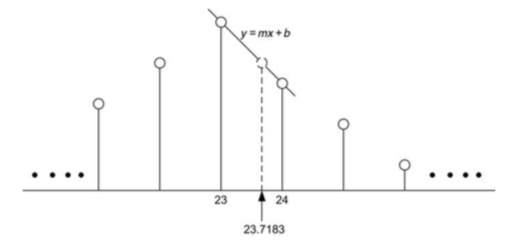
\includegraphics[width=0.8\linewidth]{assets/Linear interpolation of sample values.png}
  	\caption{Linear interpolation of sample values}
  	\label{fig:linear-interpolation}
\end{figure}



\paragraph{Polynomial Interpolation}
In polynomial interpolation a curve is drawn between the points (or a series of points), and then the interpolated value is found on that curve.~\cite{pirkle2013designing}




	\section{High-Pass Filter}\label{sec:hpf}

With high values of feedback gain and depth, we can occur in the risk of saturation, in particular at low frequencies. In order to avoid that, we decided to add a high-pass filter before the wet signal line, by implementing a first-order recursive filter:
\[
	y[n] = \alpha \cdot \left( y[n-1] + x[n] - x[n-1] \right)
	\qquad
	0 \le \alpha \le 1
\]
where $\alpha$ has the same role as the time-constant of an analog RC circuit.
In particular, it is related to the cut-off frequency $f_c$ as:
\[
	\alpha = \left( \frac{2 \pi f_c}{F_s} + 1 \right)^{-1}
\]
	\section{Interface}\label{sec:gui}

User interaction is accomplished through a simple Graphical User Interface, providing the most of the controls as sliders.
The upper area controls the LFO parameters (see section~\ref{sec:boh}). In figure~\ref{fig:gui-lfo} we can notice how the controls are always relevant to the selected waveform, i.e. for the ``random wave'' the ``phase'' slider is replaced with a ``width'' slider (see section~\ref{sec:boh} for more details on LFO parameters).

\begin{figure}[H]
	\centering
	\subcaptionbox{Sinusoidal shape}{
		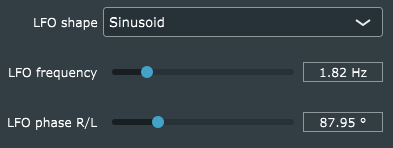
\includegraphics[width=0.5\linewidth]{assets/gui-lfo1.png}
	}%
	\subcaptionbox{Random shape}{
		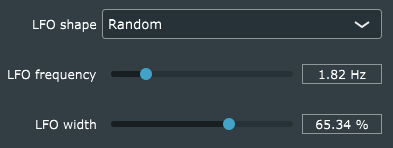
\includegraphics[width=0.5\linewidth]{assets/gui-lfo2.png}
	}
	\caption{Different parameters depending on the LFO shape}
	\label{fig:gui-lfo}
\end{figure}

The remaining controls affect the main effect parameters.

\begin{description}
	\item[Sweep width] controls the peak delay of the LFO;
	\item[Depth] controls the intensity of the effect, like a dry/wet control, and corresponds to the gain level of the delay line;
	\item[Feedback] controls the intensity of the feedback, corresponds to the gain of the feedback loop;
	\item[HP cut-off] controls the cut-off frequency of the high-pass filter;
	\item[Invert polarity] controls whether the wet signal is added or subtracted from the dry signal.
\end{description}

The full GUI as it is presented to the user is shown in figure~\ref{fig:gui-all}.

\begin{figure}
	\centering
	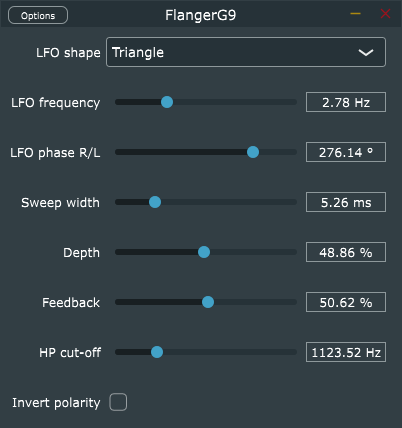
\includegraphics[width=0.5\linewidth]{assets/gui-all.png}
	\caption{Complete Graphical User Interface}
	\label{fig:gui-all}
\end{figure}

\subsection{Implementation Details}\label{sec:gui-implementation}

\nocite{juce}

In order to avoid code duplication, we adopted some techniques to define the GUI using a more descriptive approach rather than an imperative approach.

In particular, each \texttt{Slider} is dynamically generated in a \texttt{for} loop, which iterates over an array of \texttt{UISliders} objects describing the properties of each slider (i.e. label, unit, range and binding functions).
The initial \texttt{ComboBox} is populated by iterating over a \texttt{std::map} which associates each \texttt{OscFunction} enum value to the corresponding label. The final \texttt{ToggleButton}, being just one, is added directly.

Each \texttt{Component} is then added to an \texttt{Array}, which is iterated over during the \texttt{resized()} method, and laid down using a vertical main-axis \texttt{FlexBox}, to prevent hard-coding numerical values for bounds and sizes. For the styling we just kept JUCE's default \texttt{LookAndFeel}, being already clear enough for this purpose.

Value changes are bound using lambda-functions, instead of subclassing \texttt{Listener}, for easier coding.
In particular, the logic of alternating the display between the two ``phase'' and ``width'' \texttt{Slider}s is accomplished by keeping a map of ``mutually exclusive'' \texttt{Component}s. The correct \texttt{Slider} is then displayed when the \texttt{ComboBox.onChange} lambda-function is invoked.

Value unit conversion is finally performed by \texttt{FlangerProcessor}'s setter/getter methods of each parameter, following the encapsulation pattern to bridge between UI and internal representations. % interfaccia grafica
	
	\bibliographystyle{plain}
	\bibliography{bibliography}
	
\end{document}
